%%%%%%%%%%%%%%%%%%%%%%%%%%%%%%%%%%%%%%%%%
% Beamer Presentation
% LaTeX Template
% Version 1.0 (10/11/12)
%
% This template has been downloaded from:
% http://www.LaTeXTemplates.com
%
% License:
% CC BY-NC-SA 3.0 (http://creativecommons.org/licenses/by-nc-sa/3.0/)
%
%%%%%%%%%%%%%%%%%%%%%%%%%%%%%%%%%%%%%%%%%

%------------------------------------------------------------------------------------------------
%   PACKAGES AND THEMES
%------------------------------------------------------------------------------------------------

\documentclass[table, xcolor = {dvipsnames}, 9pt]{beamer}
\usepackage{tikz}
\usetikzlibrary{backgrounds}
\usetikzlibrary{arrows,shapes}
\usetikzlibrary{tikzmark}
\usetikzlibrary{calc}
\usetikzlibrary{colorbrewer}
\mode<presentation> {

% The Beamer class comes with a number of default slide themes
% which change the colors and layouts of slides. Below this is a list
% of all the themes, uncomment each in turn to see what they look like.

\usetheme{default}
%\usetheme{AnnArbor}
%\usetheme{Antibes}
%\usetheme{Bergen}
%\usetheme{Berkeley}
%\usetheme{Berlin}
%\usetheme{Boadilla}
%\usetheme{CambridgeUS}
%\usetheme{Copenhagen}
%\usetheme{Darmstadt}
%\usetheme{Dresden}
%\usetheme{Frankfurt}
%\usetheme{Goettingen}
%\usetheme{Hannover}
%\usetheme{Ilmenau}
%\usetheme{JuanLesPins}
%\usetheme{Luebeck}
%\usetheme{Madrid}
\usetheme{metropolis}
%\usetheme{Malmoe}
%\usetheme{Marburg}
%\usetheme{Montpellier}
%\usetheme{PaloAlto}
%\usetheme{Pittsburgh}
%\usetheme{Rochester}
%\usetheme{Singapore}
%\usetheme{Szeged}
%\usetheme{Warsaw}

% As well as themes, the Beamer class has a number of color themes
% for any slide theme. Uncomment each of these in turn to see how it
% changes the colors of your current slide theme.

%\usecolortheme{albatross}
%\usecolortheme{beaver}
%\usecolortheme{beetle}
%\usecolortheme{crane}
%\usecolortheme{dolphin}
%\usecolortheme{dove}
%\usecolortheme{fly}
%\usecolortheme{lily}
%\usecolortheme{orchid}
%\usecolortheme{rose}
\usecolortheme{seagull}
%\usecolortheme{seahorse}
%\usecolortheme{whale}
%\usecolortheme{wolverine}
\usefonttheme{professionalfonts}
%\setbeamertemplate{footline} % To remove the footer line in all slides uncomment this line
%\setbeamertemplate{footline}[page number] % To replace the footer line in all slides with a simple slide count uncomment this line

%\setbeamertemplate{navigation symbols}{} % To remove the navigation symbols from the bottom of all slides uncomment this line
}

\usepackage{graphicx} % Allows including images
\usepackage{booktabs} % Allows the use of \toprule, \givenrule and \bottomrule in tables
\usepackage{multirow}
\usepackage{xspace}
\usepackage{natbib}
\usepackage{hyperref}
\usepackage{diagbox}
\usepackage{makecell}
\usepackage{xparse}
\usepackage{subfig}
\usepackage{amsfonts,amsthm,amsmath,amssymb}
\usepackage{mathtools, nccmath}
\usepackage[ruled, vlined, linesnumbered]{algorithm2e}
\usepackage{wrapfig}
\usepackage{comment}  
\usepackage{bbm}
\usepackage{bm}
\usepackage{empheq}
\usepackage{pgfplots}
\usepgfplotslibrary{colorbrewer}
\usepackage{animate}
\usepackage{array}
\usepackage{ragged2e}
\newcolumntype{P}[1]{>{\RaggedRight\hspace{0pt}}p{#1}}
\newcolumntype{X}[1]{>{\RaggedRight\hspace*{0pt}}p{#1}}

% color box
\usepackage{tcolorbox}
\usepackage{tikz}
\usetikzlibrary{backgrounds}
\usetikzlibrary{arrows,shapes}
\usetikzlibrary{tikzmark}
\usetikzlibrary{calc}
% Commands for Highlighting text -- non tikz method
\newcommand{\highlight}[2]{\colorbox{#1!17}{$\displaystyle #2$}}
%\newcommand{\highlight}[2]{\colorbox{#1!17}{$#2$}}
\newcommand{\highlightdark}[2]{\colorbox{#1!47}{$\displaystyle #2$}}

% my custom colors for shading
\colorlet{mhpurple}{Plum!80}


% Commands for Highlighting text -- non tikz method
\renewcommand{\highlight}[2]{\colorbox{#1!17}{#2}}
\renewcommand{\highlightdark}[2]{\colorbox{#1!47}{#2}}

\usepgfplotslibrary{colorbrewer}

\newcommand\mybox[2][]{\tikz[overlay]\node[fill=lightgray,inner sep=2pt, anchor=text, rectangle, rounded corners=1mm,#1] {#2};\phantom{#2}}
\hypersetup{unicode=true,
            bookmarksnumbered=true,
            bookmarksopen=true,
            bookmarksopenlevel=2,
            breaklinks=false,
            pdfborder={0 0 1},
            hypertexnames=false,
            pdfstartview={XYZ null null 1}}
\usepackage{xcolor}
\hypersetup{
    colorlinks,
    linkcolor={red!50!black},
    citecolor={blue!50!black},
    urlcolor={blue!80!black}
}
\newcommand\myheading[1]{%
  \par\bigskip
  {\Large\bfseries#1}\par\smallskip}
\newcommand\given[1][]{\:#1\vert\:}
\theoremstyle{plain}
\newtheorem{thm}{Theorem}
\newtheorem{prop}{Proposition\thisthmnumber}
\newtheorem{lem}{Lemma\thisthmnumber}
\newtheorem{cor}{Corollary}
\newtheorem{defin}{Definition}
\newtheorem{algo}{Algorithm}
\newcommand*\diff{\mathop{}\!\mathrm{d}}
\newcommand*\Diff[1]{\mathop{}\!\mathrm{d^#1}}
\newcommand{\thisthmnumber}{}
\newcommand*{\QEDA}{\hfill\ensuremath{\blacksquare}}%
\newcommand*{\QEDB}{\hfill\ensuremath{\square}}%
\newcommand{\norm}[1]{\left\lVert#1\right\rVert}
\DeclareMathOperator{\N}{\mathbb{N}}
\DeclareMathOperator{\E}{\rm{E}}
\DeclareMathOperator{\R}{\mathbb{R}}
\DeclareMathOperator{\Var}{\rm{Var}}
\DeclareMathOperator{\Cov}{\rm{Cov}}
\DeclareMathOperator{\e}{\rm{e}}
\DeclareMathOperator{\logit}{\rm{logit}}
\DeclareMathOperator{\indep}{{\perp\!\!\!\perp}}
\DeclareMathOperator{\rank}{rank}
\DeclareMathOperator*{\argmin}{arg\,min}
\DeclareMathOperator*{\argmax}{arg\,max}
%\DeclareMathOperator{\Pr}{\rm{Pr}}
%------------------------------------------------------------------------
%	TITLE PAGE
%-----------------------------------------------------------------------
\pagestyle{empty}
\title[]{Introduction to Matching} % The short title appears at the bottom of every slide, the full title is only on the title page

\author{Thomas Leavitt and Ben Hansen} 
\institute[]
{

}
\date{July 26, 2024} 

\NewDocumentEnvironment{statement}{mo}
 {%
  \IfValueT{#2}{\renewcommand{\thisthmnumber}{ #2}}\begin{#1}%
 }
 {\end{#1}}

\begin{document}

\begin{frame}
\titlepage % Print the title page as the first slide
\end{frame}

%\begin{frame}
%\frametitle{Overview} % Table of contents slide, comment this block out to remove it
%\tableofcontents % Throughout your presentation, if you choose to use \section{} and \subsection{} commands, these will automatically be printed on this slide as an overview of your presentation
%\end{frame}

%-------------------------------------------------------------------------------------
%	PRESENTATION SLIDES
%-------------------------------------------------------------------------------------
\begin{frame}[t]
\frametitle{Review: Observational studies}
\vfill
\begin{itemize} \vfill
\item If any two units are the same on covariates that determine treatment assignment probabilities \vfill
\item[] $\implies$ identical propensity scores \vfill
\item Two problems with this framework \vfill
\begin{enumerate} \vfill
\item With only a few measured covariates, it is often impossible to find treated and control units exactly alike on these covariates \vfill
\item[] $\rightarrow$ \textcolor{magenta}{matching methods} \vfill
\item We usually cannot measure all relevant covariates \vfill
\item[] $\rightarrow$ \textcolor{magenta}{sensitivity analysis} \vfill
\end{enumerate}  
\end{itemize}
\vfill
\end{frame}
%-------------------------------------------------------------------------------------
\section{Matching methods}
\begin{frame}[t]
\frametitle{Matching}
\vfill
\begin{itemize} \vfill
\item Divide data into matched sets of treated and control subjects who are \textcolor{magenta}{similar} on observed covariates \vfill
\vspace{1em}
\begin{figure}
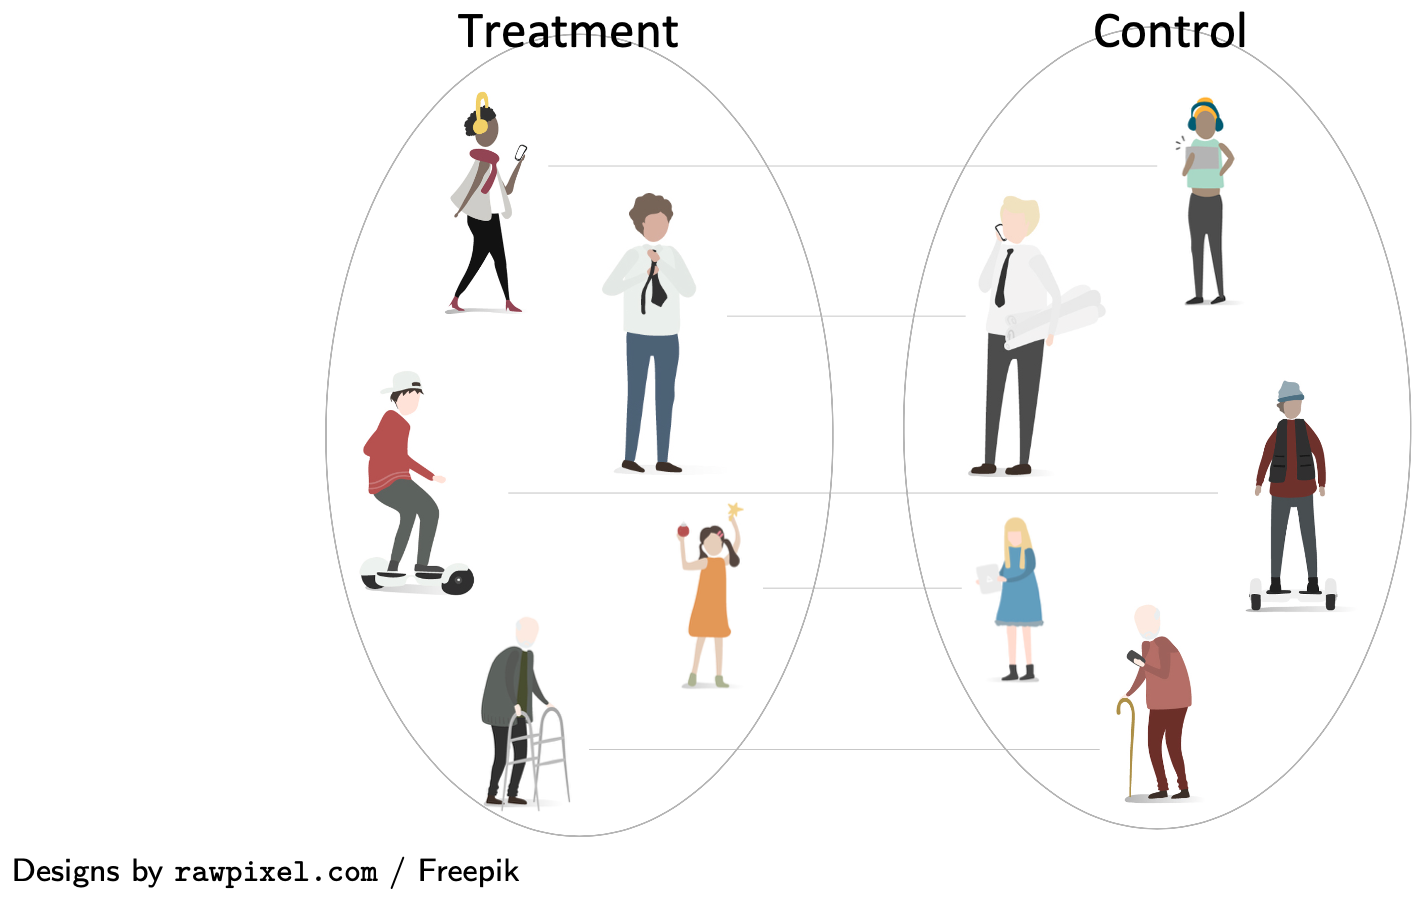
\includegraphics[width = \linewidth]{figures/matching_image.png}
\end{figure}
\vfill
\end{itemize} \vfill
\end{frame}
%-------------------------------------------------------------------------------------
\begin{frame}[t]
\frametitle{Matching: An example}
\vfill
\begin{itemize} \vfill
\item Effect of public transport system on violent crime \citep{cerdaetal2012} \vfill
\begin{itemize} \vfill
\item[] In 2004, Medell\'{i}n municipal government installed metrocables in some neighborhoods to connect them to city's urban center \vfill
\end{itemize} \vfill
\begin{figure}
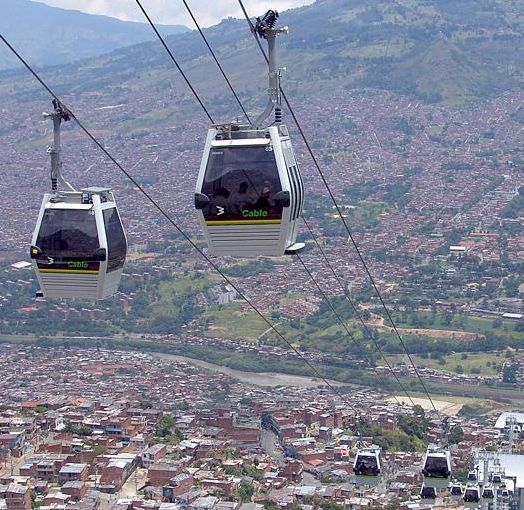
\includegraphics[width = 0.5\linewidth]{figures/medellin_metrocable.jpg}
\end{figure} \vfill
\begin{itemize} \vfill
\item Unit of analysis: Neighborhoods in Medell\'{i}n \vfill
\item Treatment variable: Metrocable or not \vfill
\item Outcome: Homicide rate \vfill
\item Covariates: Previous homicide rate, distance from city center, population size, employment rate, etc. \vfill
\end{itemize} \vfill
\end{itemize} \vfill
\end{frame}
%-------------------------------------------------------------------------------------
\begin{frame}[t]
\frametitle{Matching: An example}
\vfill
\begin{itemize} \vfill
\item What do we mean by \textcolor{magenta}{similar}? \vfill
\begin{itemize} \vfill
\item For single covariate, $x$, \textcolor{magenta}{Euclidean} distance between units $i$ and $j$ can be calculated as \vfill
\begin{align*}
\sqrt{\left(x_i - x_j\right)^2}
\end{align*} \vfill
\item For example, distance between neighborhood A (with metrocable) and neighborhood B (without) on employment rate \vfill
\begin{align*}
\sqrt{\left(0.4375 - 0.2857\right)^2} & = 0.1518
\end{align*} \vfill
\item To measure distance on many covariates, best to use  Mahalanobis distance \citep{mahalanobis1936} or Euclidean distance on \textbf{estimated} propensity score \vfill
\end{itemize} \vfill
\end{itemize} \vfill
\end{frame}
%-------------------------------------------------------------------------------------
\begin{frame}[t]
\frametitle{Matching: An example}
\vfill
\begin{table}[H]
\centering
\begin{tabular}{lll}
\hline
 & Metrocable & Employment rate \\ \hline
Neighborhood A  & 1  & 0.36 \\
Neighborhood B  & 1  & 0.25 \\
Neighborhood C  & 0  & 0.29 \\
Neighborhood D  & 0  & 0.25 \\
\hline
\end{tabular}
\end{table} \vfill
\begin{itemize} \vfill
\item How should we partition these four neighborhoods into matched sets? \vfill
\item Several ways to do so with at least one treated and one control in each set \vfill
\begin{align*}
\mathcal{M}_1 & = \left\{A, B, C, D\right\} \\
\mathcal{M}_2 & = \left\{\left\{A, C\right\}, \left\{B, D\right\}\right\} \\
\mathcal{M}_3 & = \left\{\left\{A, D\right\}, \left\{B, C\right\} \right\}
\end{align*}
\end{itemize} \vfill
\end{frame}
%-------------------------------------------------------------------------------------
\begin{frame}[t]
\frametitle{Matching: An example}
\vfill
\begin{itemize} \vfill
\item For each possible matched design, do the following \vfill
\begin{enumerate} \vfill
\item Within each matched set, calculate distance between each pair of treated and control units \vfill
\item Sum these pairwise distances within each matched set \vfill
\item Add the sums of pairwise distances over all sets \vfill
\end{enumerate} \vfill
\item \textcolor{magenta}{Optimal matching} finds matched design that minimizes this quantity
\end{itemize} \vfill
\end{frame}
%-------------------------------------------------------------------------------------
\begin{frame}[t]
\frametitle{Matching: An example}
\vfill
\begin{itemize} \vfill
\item The optimal matched design will also have a particular structure \vfill
\begin{itemize} \vfill
\item All matched sets will contains either $1$ treated unit with potentialy many control or $1$ control unit with potentially many treated units \vfill
\item This is the structure of \textbf{full matching} \citep{hansen2004} \vfill
\end{itemize} \vfill
\end{itemize} \vfill
\end{frame}
%-------------------------------------------------------------------------------------
\begin{frame}[t]
\frametitle{Matching: An example}
\vfill
\begin{table}[H]
\centering
\begin{tabular}{lll}
\hline
& Metrocable & Employment rate \\ \hline
Neighborhood A  & 1  & 0.36 \\
Neighborhood B  & 1  & 0.25 \\
Neighborhood C  & 0  & 0.29 \\
Neighborhood D  & 0  & 0.25 \\
\hline
\end{tabular}
\end{table} \vfill
\begin{itemize}
\item $\mathcal{M}_1 = \left\{A, B, C, D\right\}$ \vfill
\footnotesize
\begin{align*}
\sqrt{\left(0.36 - 0.29\right)^2} + \sqrt{\left(0.36 - 0.25\right)^2} + \sqrt{\left(0.25 - 0.29\right)^2} + \sqrt{\left(0.25 - 0.25\right)^2} = 0.22
\end{align*} \vfill
\normalsize
\item $\mathcal{M}_2 = \left\{\left\{A, C\right\}, \left\{B, D\right\}\right\}$ \vfill
\footnotesize
\begin{align*}
\left(\sqrt{\left(0.36 - 0.29\right)^2}\right) + \left(\sqrt{\left(0.25 - 0.25\right)^2}\right) = 0.07
\end{align*} \vfill
\normalsize
\item $\mathcal{M}_3 = \left\{\left\{A, D\right\}, \left\{B, C\right\} \right\}$ \vfill
\footnotesize
\begin{align*}
\left(\sqrt{\left(0.36 - 0.25\right)^2}\right) + \left(\sqrt{\left(0.25 - 0.29\right)^2}\right) = 0.15
\end{align*} \vfill
\normalsize
\item[] \vfill 
\textcolor{magenta}{$\mathcal{M}_2 = \left\{\left\{A, C\right\}, \left\{B, D\right\}\right\}$ is best match} \vfill
\end{itemize} \vfill
\end{frame}
%-------------------------------------------------------------------------------------
\begin{frame}[t]
\frametitle{Matching: An example}
\vfill
\begin{itemize}
\item With many covariates, follow same procedure but with multivariate distance measure \vfill
\item In practice, optimal matching implemented via statistical software, \texttt{optmatch} in \texttt{R} \vfill
\item Can impose additional restrictions that forbid certain matches \vfill
\begin{itemize} \vfill
\item E.g., cannot put in same set any two neighborhoods that are more than $0.05$ apart on employment rate \vfill
\item With such restrictions, may end up dropping units from analysis \vfill
\end{itemize} \vfill
\end{itemize} \vfill
\end{frame}
%-------------------------------------------------------------------------------------
\begin{frame}[t]
\frametitle{Matching: An example}
\vfill
\begin{itemize} \vfill
\item To estimate and test hypotheses about effects after matching \vfill
\begin{itemize} \vfill
\item Estimate ATE within each matched set and then average over all estimates, weighting by proportion of units in each set \vfill
\end{itemize} \vfill
\item For example, suppose partition of 45 Medell\'{i}n neighborhoods into $6$ matched sets \vfill
 \begin{table}[H]
\centering
\begin{tabular}{lll}
\hline
Matched set & Number of units & Difference-in-Means \\ \hline
A & 14 & -0.136  \\
B & 2  & -0.115 \\
C & 19 & -0.486 \\
D & 3  & -0.164 \\
E & 2  & -0.0547 \\
F & 5  & 0.0263 \\
\hline
\end{tabular}
\end{table} \vfill
\item Overall estimate is \vfill
\footnotesize
\begin{align*}
-\left(14/45\right)0.136 - \left(2/45\right)0.115 - \left(19/45\right)0.486 & \\
- \left(3/45\right)0.164 - \left(2/45\right)0.0547 + \left(5/45\right)0.0263 \\ 
& \approx -0.26 
\end{align*}
\normalsize
\end{itemize} \vfill
\end{frame}
%-------------------------------------------------------------------------------------
\begin{frame}[allowframebreaks]
\frametitle{References} 
\scriptsize
\bibliographystyle{chicago}
\bibliography{Bibliography.bib}   % name your BibTeX data base
\end{frame}
%-------------------------------------------------------------------------------------
\end{document}